\section{Experimentación y entorno de ejecución}

En esta sección se detallará el entorno de pruebas junto con las justificaciones de las elecciones realizadas a lo largo de la experimentación. Para el desarrollo del código se usa el lenguaje Python principalmente con las librerías PyTorch, FastAI, Numpy, SKlearn y Pandas; implementado y ejecutado en la plataforma Paperspace, que proporciona un IDE y un entorno de ejecución online similar a Google Colab, pero en el que podemos elegir manualmente el hardware sobre el que ejecutamos el código, de manera que la comparación de tiempos y recursos entre las distintas técnicas sea objetiva. El hardware usado es Nvidia Quadro P5000, proporcionado por la plataforma. El código puede encontrarse en: \url{https://github.com/eedduu/TFG}. 

En la tabla \ref{table:exp} encontramos un esquema de los experimentos a realizar. Dada la cantidad de modelos distintos que vamos a entrenar, se ha decidido dividir el código en un archivo por tarea, teniendo cada conjunto de datos su propio archivo \verb|conjunto_de_datos.ipynb|. Se ha elegido este formato de archivo en lugar de \verb|conjunto_de_datos.py| de manera que se puedan comprobar las salidas del proyecto fácilmente. Se ha creado un módulo de python llamado \verb|utilsTFG.py| que contiene funciones comunes al código, como métricas de error propias, herramientas para el preprocesado de datos, los modelos ConvNets, funciones para graficar resultados o los algoritmos metaheurísticos. También hay un archivo \verb|comparative.ipynb| donde se realizan comparativas a posteriori de los resultados, como por ejemplo graficar relaciones entre los rendimientos de algunas técnicas o llevar a cabo test estadísticos.





\begin{table}[]
\resizebox{\textwidth}{!}{\begin{tabular}{|l|cccc|cll|}
\hline
\textbf{Familia} & \multicolumn{4}{c|}{MLP}                                                                                                                               & \multicolumn{3}{c|}{ConvNets}                                         \\ \hline
\textbf{Modelo}  & \multicolumn{4}{c|}{1,2,5 y 11}                                                                                                                        & \multicolumn{3}{c|}{LeNet5, ResNet-15 y ResNet57}                               \\ \hline
\textbf{conjuntos de datos}           & \multicolumn{1}{c|}{BHP} & \multicolumn{1}{c|}{BCW} & \multicolumn{2}{c|}{WQ}              & \multicolumn{1}{c|}{MNIST} & \multicolumn{1}{l|}{F-MNIST} & CIFAR10-G \\ \hline
\textbf{Tarea}             & \multicolumn{1}{c|}{R}                        & \multicolumn{1}{c|}{C}            & \multicolumn{1}{c|}{R} & C & \multicolumn{3}{c|}{Clasificación de imágenes}                        \\ \hline
\end{tabular}}
\caption{Resumen de la experimentación. BHP: Boston Housing Price, BCW: Breast Cancer Winsconsin, WQ: Wine Quality. R: regresión, C: clasificación. En el caso de MLP, en la fila modelo se indica el número de capas ocultas.}
\label{table:exp}
\end{table}


\subsection{Reproducibilidad}

En todas las funciones y librerías usadas en las que intervienen generación de números aleatorios se fija el valor de su semilla a 42. Esto se hace al iniciarse el proyecto, de manera que afecte a la separación de los datos en entrenamiento, de test y a la generación de parámetros iniciales para los modelos que vamos a entrenar con gradiente descendente. Luego se vuelve a fijar la semilla para todas las librerías que corresponda para generar la población que usaremos con las técnicas metaheurísticas y se fija también de nuevo antes de iniciar cada entrenamiento, de manera que se puedan repetir los experimentos por separado.

Esto último también se realiza ya que la experimentación ha debido realizarse en ejecuciones separadas, y fijando la semilla de nuevo obtenemos el mismo estado para los generadores de números aleatorios, con lo que no tenemos problema al dividir las ejecuciones. Se han guardado además, a través de la librería \verb|pickle|, tanto las poblaciones iniciales como los modelos y tiempos obtenidos para cada tarea, de manera que estos son comprobables.







\subsection{Modelos}

Usaremos dos familias de modelos: MLP y ConvNets. Con los primeros usaremos conjuntos de datos tabulares para clasificación y regresión, y con los segundos conjuntos de datos de imágenes para la tarea de clasificación. La implementación de los MLP se ha realizado a través de la librería FastAI por simplicidad ya que ofrece lo necesario para usarlos directamente. La implementación de las ConvNets se ha realizado desde cero, observando la topología de LeNet5 y las ResNets en sus papers originales, ya que en ellas sí que se han introducido ciertos cambios que se comentan más adelante. Todos los modelos han sido entrenados desde cero.

Usaremos 4 modelos de tipo MLP, con 1,2,5 y 11 capas ocultas cada uno. El número de neuronas por capa es una potencia de 2 y con estructura piramidal incremental, es decir primero aumentando el número de neuronas por capa y luego disminuyéndolo. Estas son elecciones comunes en la literatura ya que facilitan las operaciones por su estructura (la primera) y el tratamiento de los datos (la segunda).

\begin{table}[]
\centering
\begin{tabular}{|c|c|c|}
\hline
\textbf{Capas ocultas} & \textbf{Neuronas por capa}                                                                     & \textbf{Parámetros} \\ \hline
1                      & 64                                                                                             & 2238                \\ \hline
2                      & 64, 64                                                                                         & 6462                \\ \hline
5                      & 64, 128, 256, 128, 64                                                                          & 85k                 \\ \hline
11                     & \begin{tabular}[c]{@{}c@{}}32, 64, 128, 256, 512, 1024, \\ 512, 256, 128, 64 y 32\end{tabular} & 1.4M                \\ \hline
\end{tabular}
\caption{Detalles de los modelos MLP}
\label{tab:MLPmod}
\end{table}

Antes de cada capa linal hay una capa BatchNorm1D, ya que es la implementación por defecto de FastAI y mejora el rendimiento en el entrenamiento. Los parámetros asociados a este tipo de capa y a los de la capa de salida van incluidos en el cómputo anterior. Se incluye al final del modelo una capa de \textit{SoftMax} en caso de que la tarea sea clasificación.

Para los modelos basados en convoluciones usamos LeNet5 y dos ResNets, con 15 y 57 capas. En el primero sustituimos las funciones de activación por ReLU, ya que en la literatura posterior a la presentación del modelo se han demostrado superiores a las sigmoides y la tangente hiperbólica. También se han sustituido las capas de \textit{AveragePool} por \textit{MaxPool} y añadido capas de BatchNorm por los mismos motivos. En la tabla \ref{table:lenet5} se muestra la topología de este modelo, obviando las capas de \textit{Flatten} y de \textit{SoftMax}. Tiene un total de 62 mil parámetros.



\begin{table}[]
\centering
\begin{tabular}{|c|c|c|c|}
\hline
\multirow{2}{*}{\textbf{Capa}} & \multirow{2}{*}{\textbf{Dimensión}} & \multirow{2}{*}{\textbf{Kernel}} & \multirow{2}{*}{\textbf{Canales}} \\
                               &                                     &                                  &                                   \\ \hline
Convolución                    & 28x28                               & 5x5                              & 6                                 \\ \hline
BatchNorm2D                    & 28x28                               & -                                & -                                 \\ \hline
ReLU                           & 28x28                               & -                                & -                                 \\ \hline
Max Pool                       & 14x14                               & 2x2, stride 2                    & -                                 \\ \hline
Convolución                    & 10x10                               & 5x5                              & 16                                \\ \hline
BatchNorm2D                    & 10x10                               & -                                & -                                 \\ \hline
ReLU                           & 10x10                               & -                                & -                                 \\ \hline
Max Pooling                    & 5x5                                 & 2x2                              & -                                 \\ \hline
Lineal                         & 120                                 & -                                & -                                 \\ \hline
BatchNorm1D                    & 120                                 & -                                & -                                 \\ \hline
ReLU                           & 120                                 & -                                & -                                 \\ \hline
Lineal                         & 84                                  & -                                & -                                 \\ \hline
BatchNorm1D                    & 84                                  & -                                & -                                 \\ \hline
ReLU                           & 84                                  & -                                & -                                 \\ \hline
Lineal                         & num\_classes                        & -                                & -                                 \\ \hline
\end{tabular}
\caption{Topología de LeNet5 para imágenes 32x32 con un canal de entrada. Las columnas dimensión y canales hacen referencia a la salida de la capa.}
\label{table:lenet5}
\end{table}


Se han diseñado dos modelos de ResNet, uno con 15 capas y otro con 57. Los bloques convolucionales agrupan 3 capas de convolución con sus respectivas capas BatchNorm, y se usan convoluciones 1x1 para hacer cuello de botella, reduciendo así el número de parámetros sin perder expresividad de la red. Se sigue el diseño usual de esta familia de modelos, por ejemplo agrupando más bloques convolucionales en mitad de la red, con una convolución previa a los bloques convolucionales y usando solo una capa lineal. El modelo ResNet57 que se implementa tiene un total de 1.3M de parámetros, mientras que ResNet15 tiene 500 mil. Sus topologías pueden observarse en las tablas \ref{table:resnet57} y \ref{table:resnet15} respectivamente. 

\begin{table}[]
\begin{tabular}{|c|c|c|c|}
\hline
\multirow{2}{*}{\textbf{Capa}} & \multirow{2}{*}{\textbf{Dimensión}} & \multirow{2}{*}{\textbf{Kernel/Stride}} & \multirow{2}{*}{\textbf{Canales}} \\
                               &                                            &                                         &                                          \\ \hline
Convolución                    & 26x26                                      & 7x7                                     & 64                                       \\ \hline
BatchNorm2d                    & 26x26                                      & -                                       & -                                        \\ \hline
ReLU                           & 26x26                                      & -                                       & -                                        \\ \hline
MaxPool2d                      & 13x13                                      & 2x2, stride 2, padding 1                & -                                        \\ \hline
BottleneckBlock x3             & 13x13                                      & 1x1, 3x3, 1x1                           & 64                                       \\ \hline
BottleneckBlock x4             & 7x7                                        & 1x1, 3x3, 1x1, stride 2                 & 128                                      \\ \hline
BottleneckBlock x4             & 4x4                                        & 1x1, 3x3, 1x1, stride 2                 & 256                                      \\ \hline
BottleneckBlock x3             & 2x2                                        & 1x1, 3x3, 1x1, stride 2                 & 512                                      \\ \hline
AdaptiveAvgPool2d              & 512                                        & -                                       & -                                        \\ \hline
BatchNorm1d                    & 512                                        & -                                       & -                                        \\ \hline
Dropout                        & 512                                        & -                                       & -                                        \\ \hline
Lineal                         & num\_classes                               & -                                       & -                                        \\ \hline
\end{tabular}
\caption{Topología de ResNet57 para imágenes 32x32 con un canal de entrada. Las columnas dimensión y canales hacen referencia a la salida de la capa.}
\label{table:resnet57}
\end{table}


\begin{table}[]
\begin{tabular}{|c|c|c|c|}
\hline
\multirow{2}{*}{\textbf{Capa}} & \multirow{2}{*}{\textbf{Dimensión}} & \multirow{2}{*}{\textbf{Kernel/Stride}} & \multirow{2}{*}{\textbf{Canales}} \\
                               &                                     &                                         &                                   \\ \hline
Convolución                    & 26x26                               & 7x7                                     & 64                                \\ \hline
BatchNorm2d                    & 26x26                               & -                                       & -                                 \\ \hline
ReLU                           & 26x26                               & -                                       & -                                 \\ \hline
MaxPool2d                      & 13x13                               & 2x2, stride 2, padding 1                & -                                 \\ \hline
BottleneckBlock x1             & 13x13                               & 1x1, 3x3, 1x1                           & 64                                \\ \hline
BottleneckBlock x1             & 7x7                                 & 1x1, 3x3, 1x1, stride 2                 & 128                               \\ \hline
BottleneckBlock x1             & 4x4                                 & 1x1, 3x3, 1x1, stride 2                 & 256                               \\ \hline
BottleneckBlock x1             & 2x2                                 & 1x1, 3x3, 1x1, stride 2                 & 512                               \\ \hline
AdaptiveAvgPool2d              & 512                                 & -                                       & -                                 \\ \hline
BatchNorm1d                    & 512                                 & -                                       & -                                 \\ \hline
Dropout                        & 512                                 & -                                       & -                                 \\ \hline
Lineal                         & num\_classes                        & -                                       & -                                 \\ \hline
\end{tabular}
\caption{Topología de ResNet15 para imágenes 32x32 con un canal de entrada. Las columnas dimensión y canales hacen referencia a la salida de la capa.}
\label{table:resnet15}
\end{table}


Estos modelos se han elegido con el objetivo de tener una gama experimental amplia en base al número de parámetros, de manera que nos permita responder de manera adecuada al punto 2 de las cuestiones \textit{P1} y \textit{P2} que nos planteábamos en \ref{sec:objinf}. 


\subsection{Conjuntos de datos} \label{sec:conjuntos_de_datos}

Hemos elegido 3 conjuntos de datos de clasificación de imágenes usados en \cite{MHtrainingClase}, de manera que los experimentos sean comparables. Para las tareas con MLP hemos elegido tres conjuntos de datos tabulares, aunque uno de ellos (WQ) es usado para dos tareas distintas: regresión y clasificación, teniendo por tanto cuatro tareas. Se han elegido estos conjuntos de datos en base a su número de citas, su tarea y la adecuación de sus características a la batería experimental.

La intención con la elección de estos conjuntos de datos es poder responder a las cuestiones:

\begin{itemize}

\item \textit{P1,P2}. Los diferentes tamaños de los conjuntos de datos seleccionados (desde 500 hasta 15 mil), y las diferentes complejidades de las tareas asociadas (desde muy fáciles hasta complejidad media-alta) nos hacen poder responder a los puntos 1 y 3 de los análisis del rendimiento y complejidad computacional.

\item \textit{P3}. Para tareas con MLP, se han elegido dos tareas de clasificación y dos de regresión.

\end{itemize} 







\subsubsection{Tabulares}

\begin{table}[]
\centering
\begin{tabular}{|c|c|c|c|}
\hline
\textbf{Conjunto de datos}            & \textbf{BCW} & \textbf{BHP} & \textbf{WQ} \\ \hline
\textbf{Tarea}              & C            & R            & C y R       \\ \cline{1-1}
\textbf{Nº instancias}      & 569          & 506          & 1143        \\ \cline{1-1}
\textbf{Nº características} & 30           & 13           & 11          \\ \cline{1-1}
\textbf{Objetivo}           & Diagnosis    & MEDV         & Quality     \\ \cline{1-1}
\textbf{Ratio balance}      & 1.68         & -            & 80.5        \\ \cline{1-1}
\textbf{Faltan valores}     & No           & Si           & No          \\ \cline{1-1}
\textbf{Complejidad}        & Media-baja   & Media-baja        & Media-alta  \\ \hline
\end{tabular}
\caption{Información sobre los conjuntos de datos tabulares. El ratio de balance se calcula dividiendo el número de instancias de la clase más usual entre la menos usual. BCW: Breast Cancer Winsconsin, BHP: Boston Housing Price, WQ: Wine Quality. C: clasificación, R: regresión.}
\label{tab:dat_tab}
\end{table}
En la tabla \ref{tab:dat_tab} podemos ver un resumen de estos conjuntos de datos. Vamos a describirlos un poco más en profundidad:

\begin{itemize}

\item BCW \footnote{\url{https://www.kaggle.com/conjuntos de datos/uciml/breast-cancer-wisconsin-data}}: las características se calculan a partir de una imagen digitalizada de un aspirado con aguja fina de una masa mamaria. Describen las características de los núcleos celulares presentes en la imagen. Se extraen diez características como el radio, perímetro, área, etc. y de cada una de ellas se calcula la media, la desviación estándar y la peor, resultando en las 30 características finales. El objetivo a clasificar es binario, el diagnóstico puede resultar beningno o maligno. 

\item BHP\footnote{\url{https://www.kaggle.com/conjuntos de datos/altavish/boston-housing-conjunto de datos}}: se obtiene a partir de datos sobre el mercado de la vivienda en Boston. Sus características describen varios factores como los impuestos sobre cada vivienda o la tasa de criminalidad en el barrio. El objetivo a predecir es MEDV (\textit{Median Value}), es decir el valor mediano de las casas habitadas en escala de mil dólares.

\item WQ \footnote{\url{https://www.kaggle.com/conjuntos de datos/yasserh/wine-quality-conjunto de datos}}: describe varias características del vino en base a tests fisico-químicos como la densidad, el pH o los sulfatos que contiene. Debemos predecir la calidad (1-10) mediante clasificación o regresión. La mayor complejidad reside en el poco balance entre las clases a predecir.

\end{itemize}

Para estos conjuntos de datos se ha realizado un preprocesado de los datos básico y con decisiones comunes basadas en la literatura. Se han eliminado las variables que tienen menos de un 5 o 10\% (dependiendo de la cantidad de variables del conjunto de datos) de correlación con la variable objetivo. Con las parejas de variables que tienen más de un 90\% de correlación entre sí se elimina una de las dos. Se han eliminado outliers con el método \textit{zscore} y se han escalado los datos de entrada a través de la normalización. El tamaño del batch se ha elegido mediante pruebas experimentales entre los valores 32, 64 y 128. Se divide el conjunto de datos en entrenamiento-validación-test, con un porcentaje 70-10-20. 



\subsubsection{Imágenes}

Usamos como conjuntos de datos MNIST\footnote{\url{https://yann.lecun.com/exdb/mnist/}}, F-MNIST\footnote{\url{https://www.kaggle.com/conjunto de datoss/zalando-research/fashionmnist}} y CIFAR-10\footnote{\url{https://www.kaggle.com/c/cifar-10/}}. Se reducen a 10 mil imágenes para el conjunto de entrenamiento, del cual se toman 3 mil para validación; y 5 mil para test. Nos aseguramos de que las clases sigan perfectamente balanceadas después de la reducción. Se usan las imágenes con una resolución de 32x32 y un solo canal de escala de grises, adaptando las imágenes a estas dimensiones cuando sea necesario. No se realiza preprocesamiento de datos ya que se entiende que la propia red a través de las convoluciones realiza las transformaciones necesarias. Estas elecciones se realizan, al igual que la elección del tamaño del batch, para establecer un marco común con el paper de referencia. La decisión de tomar la partición de validación del conjunto de entrenamiento corresponde principalmente a reducir el tamaño del mismo debido a las limitaciones de memoria del hardware y a la necesidad de tener un conjunto de validación (a diferencia del paper de referencia) debido a que sólo realizamos una ejecución del entrenamiento.

Vamos a conocer un poco más estos conjuntos de datos. MNIST contiene imágenes de resolución $28 \times 28$ de dígitos manuscritos (0-9) como se muestra en la figura \ref{fig:mnist}. Su complejidad es baja debido a la simplicidad de las imágenes (baja resolución y escala de grises) y la naturaleza bien definida de los dígitos, habiendo poca variabilidad en los datos. Es un \textit{benchmark} estandarizado para algoritmos de clasificación de imágenes sencillos.

\begin{figure}
    \centering
    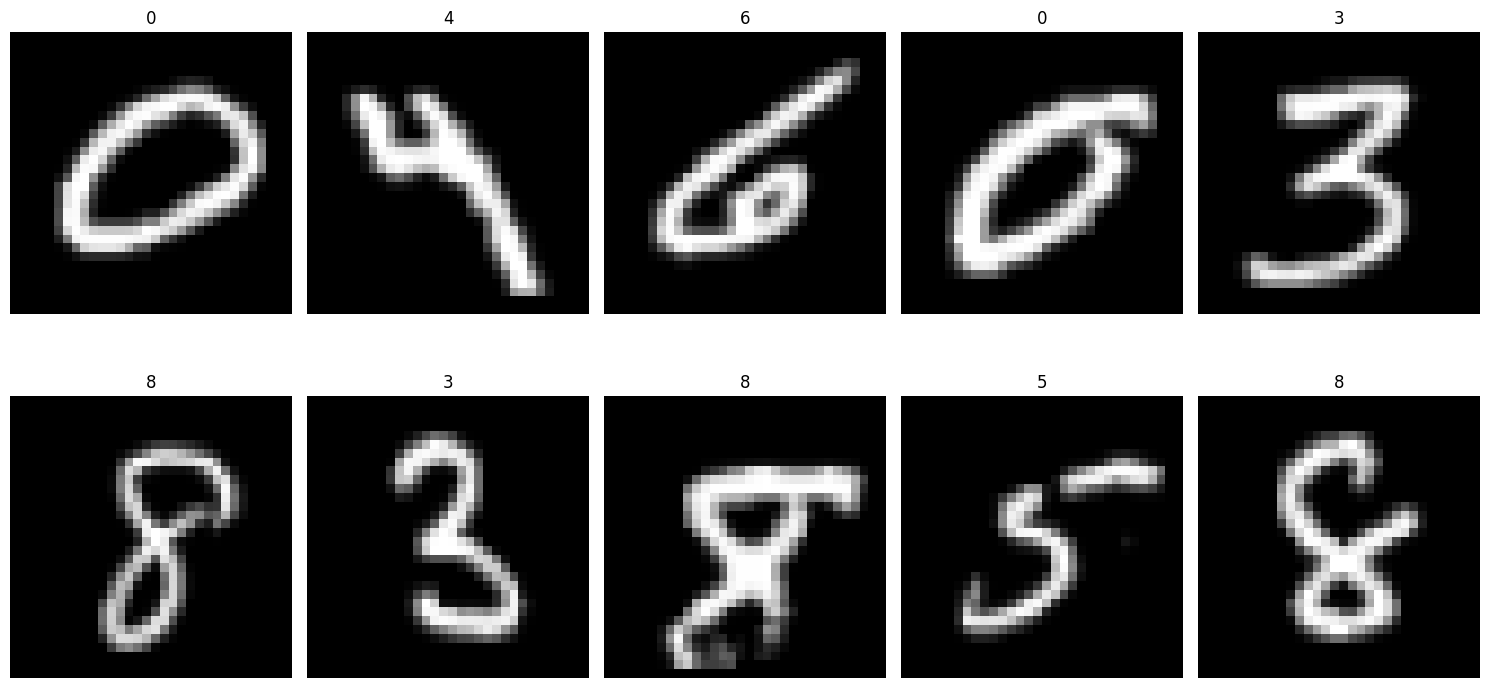
\includegraphics[width=0.75\linewidth]{Plantilla_TFG_latex//imagenes//Inf//exp/mnist.png}
    \caption{Ejemplo de 10 imágenes aleatorias del conjunto de entrenamiento de MNIST, con sus respectivas etiquetas.}
    \label{fig:mnist}
\end{figure}

F-MNIST por su parte tiene imágenes en escala de grises de 10 tipos de ropa distintos (por ejemplo pantalones, camisetas, zapatos) como vemos en la imagen \ref{fig:fmnist}, con la misma resolución que MNIST pero una complejidad media-baja. Esta diferencia se debe principalmente a la mayor variabilidad en los objetos de ropa y sus características. Las imágenes son más complejas y tienen patrones más intrincados que los dígitos.

\begin{figure}
    \centering
    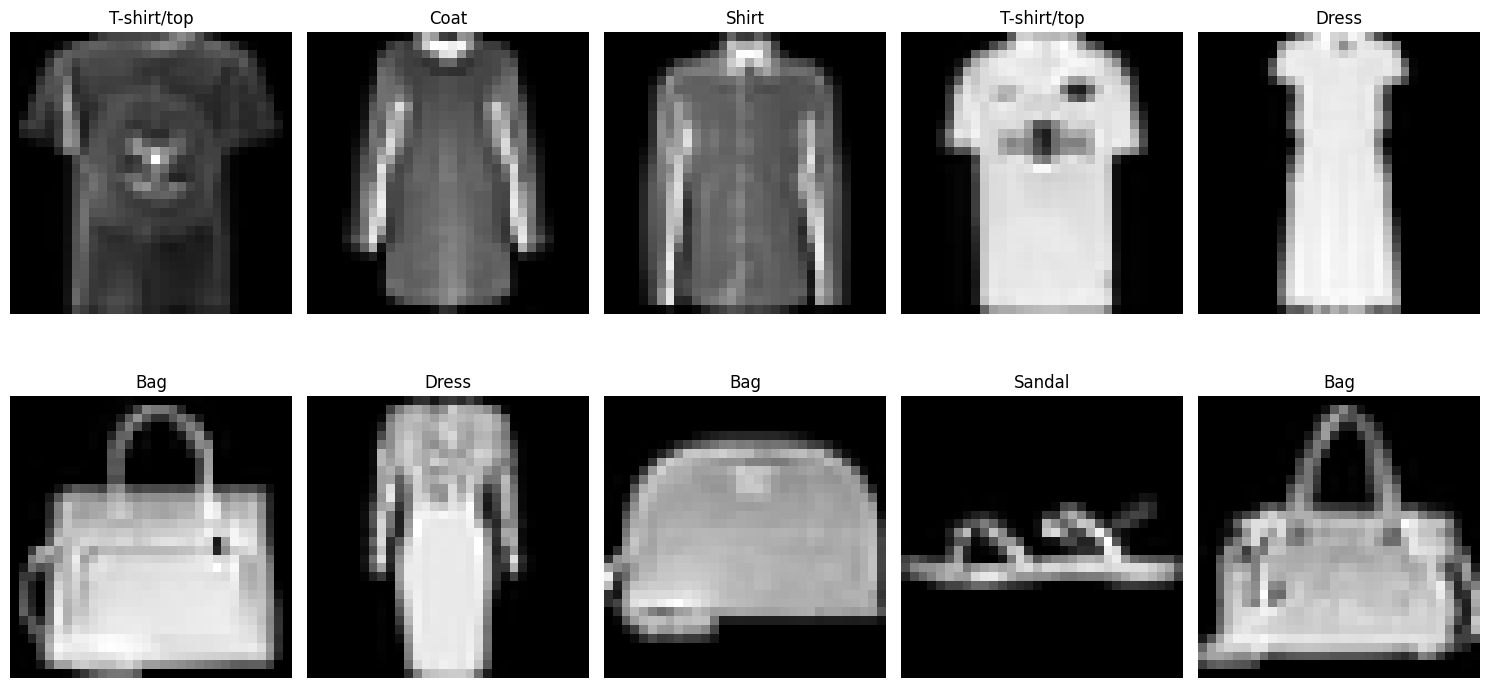
\includegraphics[width=0.75\linewidth]{Plantilla_TFG_latex//imagenes//Inf//exp/fmnist.png}
    \caption{Ejemplo de 10 imágenes aleatorias del conjunto de entrenamiento de F-MNIST, con sus respectivas etiquetas.}
    \label{fig:fmnist}
\end{figure}

Por último CIFAR-10 contiene imágenes en resolución $32 \times 32 \times 3$, aunque las convertimos a un solo canal en escala de grises como podemos ver en la figura \ref{fig:cifar10}, por lo que nos referimos a este conjunto de datos como CIFAR-10-G. Incluye 10 clases de objetos como aviones, coches, pájaros, gatos, etc. La complejidad es alta debido a la naturaleza de las imágenes, que contienen una amplia variedad de objetos con diferentes formas, texturas y fondos. Las imágenes son relativamente pequeñas en resolución para la cantidad de información contenida en ellas, haciendo más difídil distinguir pequeños detalles necesarios para una correcta clasificación. La variabilidad en los datos requiere de técnicas más avanzadas para clasificación, haciéndolo un \textit{benchmark} estandarizado para evaluar modelos de aprendizaje profundo. Reducir las imágenes a un solo canal ayuda a reducir la cantidad de parámetros del modelo y el tiempo de entrenamiento, pero para saber si afecta a la complejidad de la tarea habría que realizar un análisis específico, ya que aunque perdemos información sobre los datos no está claro que sea información relevante. Para ello, por ejemplo, los colores deberían ser consistentes dentro de una misma clase, y diferentes a los colores de las demás.

\begin{figure}
    \centering
    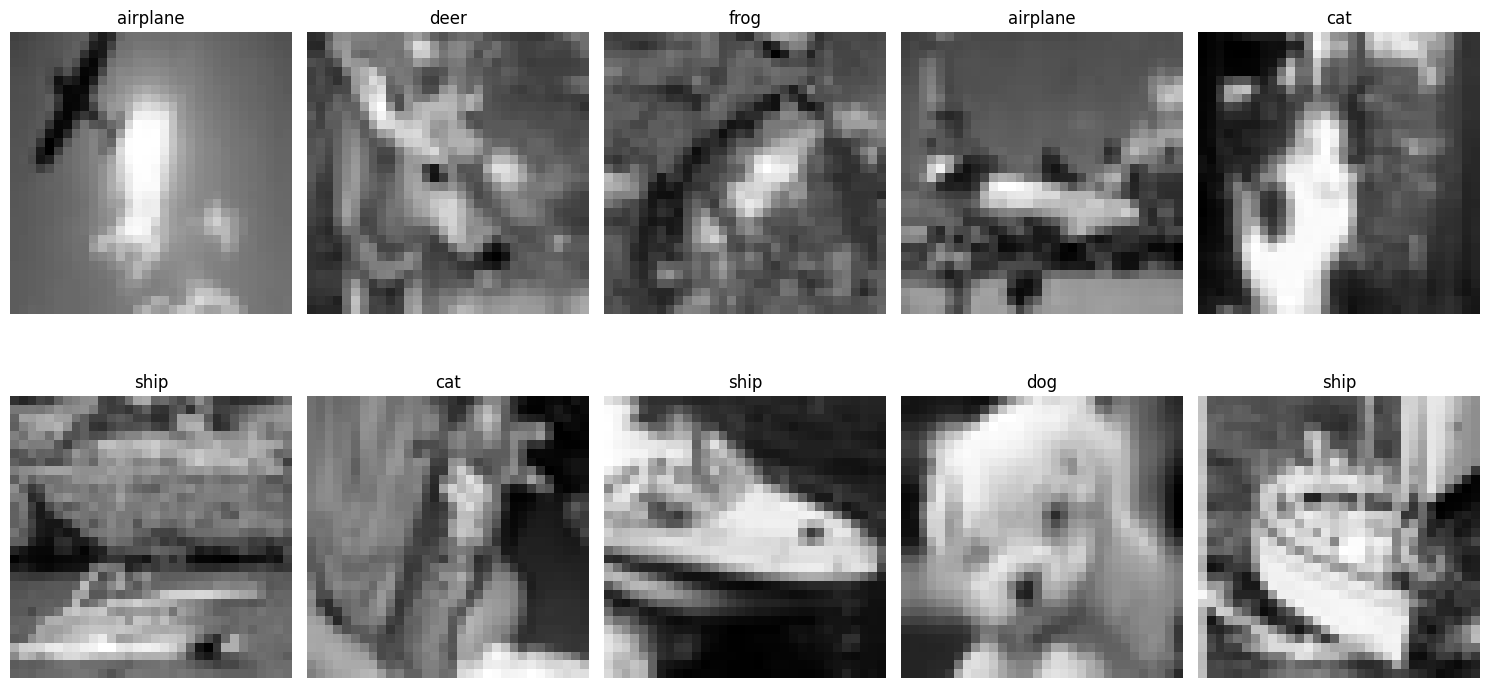
\includegraphics[width=0.75\linewidth]{Plantilla_TFG_latex//imagenes//Inf//exp/cifar10.png}
    \caption{Ejemplo de 10 imágenes aleatorias del conjunto de entrenamiento de CIFAR-10-G, con sus respectivas etiquetas.}
    \label{fig:cifar10}
\end{figure}


\subsection{Entrenamiento}

Usamos los tres optimizadores de primer orden de gradiente descendente mencionados anteriormente con un doble objetivo. En primer lugar así tenemos resultados más diversos con los que comparar las técnicas metaheurísticas, pudiendo observar si estos algoritmos mejoran a alguno o ninguno de los optimizadores propuestos. Como los tres optimizadores son ampliamente usados en la literatura, creemos que esta información es pertinente. Por otro lado, sabemos que el optimizador que mejores resultados consiga depende ampliamente de la tarea y del modelo, por tanto, al ejecutar las técnicas hibridadas con el gradiente descendente podemos asignar a cada modelo el optimizador que mejor rendimiento haya ofrecido en la tarea.

En las estrategias metaheurísticas elegimos usar SHADE y SHADE-ILS. El primero es uno de los algoritmos sin búsqueda local que mejores resultados ofrece en optimización de problemas continuos, mientras que el segundo es un referente en la optimización de problemas continuos a gran escala y especialmente en el entrenamiento de modelos. Además proponemos dos técnicas nuevas: SHADE-GD y SHADE-ILS-GD, que resultan de la hibridación de las anteriores con el gradiente descendente. Estas decisiones nos permiten responder directamente a la cuestión \textit{P4}, mientras que la comparativa entre estos dos enfoques es necesaria para responder al resto.

Debido a la sensibilidad del entrenamiento a los parámetros iniciales, se han usado los mismos pesos iniciales para los entrenamientos con distintos optimizadores de un mismo modelo. De manera similar, se usa la misma población inicial de soluciones para un mismo modelo en cada entrenamiento con técnicas metaheurísticas. Se ha usado la inicialización de pesos Glorot, al igual que en el paper de referencia. Como diferencia respecto a dicha publicación, no usamos validación cruzada por los excesivos recursos computacionales que supondría, con lo que dividimos los datos en entrenamiento-validación-test tal como se indica en \ref{sec:conjuntos_de_datos}.

Para las tareas de regresión se ha usado el error cuadrático medio como función de coste. Es ampliamente usada en la literatura y aunque es sensible a los valores extremos, como tenemos preprocesamiento de datos vemos reducido el efecto. Se ha usado también la métrica R$^2$ para medir la explicación de la varianza con respecto a la media como predicción, para tener un criterio objetivo de comparación ya que en las dos tareas de regresión la escala del objetivo es distinta. Para las tareas de clasificación se ha usado la entropía cruzada como función de error y \textit{accuracy} como métrica, opciones ampliamente usadas en la literatura. En los conjuntos de datos tabulares se ha usado \textit{BalancedAccuracy} en lugar de \textit{accuracy}, ya que las clases no están balanceadas, y se conoce que en estos casos la segunda no es una métrica representativa, de hecho se hace especial mención a esto en \cite{MHtrainingClase}. En los conjuntos de datos de imágenes las clases están perfectamente balanceadas por lo que se usa \textit{accuracy}, aunque en este caso su versión balanceada coincidiría con la normal.

Para la elección de hiperparámetros usamos los elegidos en \cite{MHtrainingClase}, en los casos en que no podamos basarnos en el paper, usaremos los valores por defecto de PyTorch y los propuestos en los papers originales, en ese orden. Estos valores predeterminados de PyTorch, aunque no conseguirán el mejor rendimiento posible, están optimizados para funcionar bien en una variedad muy amplia de situaciones. Además el propósito es una comparación objetiva entre las técnicas de entrenamiento, no obtener el máximo rendimiento de cada una de ellas. Debido al gran número de modelos que entrenamos, no podríamos invertir el tiempo necesario para ajustar correctamente todos los hiperparámetros, en especial los referentes a los algoritmos metaheurísticos. Podemos ver los valores usados en la tabla \ref{tab:params}.

% Please add the following required packages to your document preamble:
% \usepackage{multirow}
\begin{table}[]
\centering
\begin{tabular}{cccc}
\multicolumn{2}{c}{}                                          & \textbf{Parámetro} & \textbf{Valor} \\ \hline
\multicolumn{2}{c}{\multirow{2}{*}{\textbf{Comunes}}}         & Pesos iniciales    & Glorot         \\
\multicolumn{2}{c}{}                                          & Épocas             & 20             \\ \hline
\multirow{4}{*}{\textbf{GD}} & \multirow{2}{*}{\textbf{ADAM}} & $\beta_1$          & 0.9            \\
                             &                                & $\beta_2$          & 0.999          \\
                             & \textbf{RMSPROP}               & $\alpha$           & 0.99           \\
                             & \textbf{NAG}                   & mom                & 0.9            \\ \hline
\multicolumn{2}{c}{\multirow{6}{*}{\textbf{MH}}}              & N$_{pob}$          & 10             \\
\multicolumn{2}{c}{}                                          & Max\_evals         & 4200           \\
\multicolumn{2}{c}{}                                          & Evals$_{SHADE}$    & 200            \\
\multicolumn{2}{c}{}                                          & Evals$_{LS}$       & 10             \\
\multicolumn{2}{c}{}                                          & Reinicio           & 3              \\
\multicolumn{2}{c}{}                                          & \% mejora          & 5              \\ \hline
\end{tabular}
\caption{}
\label{tab:params}
\end{table}

\subsubsection{Gradiente descendente}

El criterio para elegir los tres optimizadores ha sido el siguiente: en primer lugar decidimos incorporar tres técnicas basadas en gradiente descendente para tener diversidad en los resultados, como se expone arriba, y en concreto ese es el número de estrategias distintas en los que se dividen a granden rasgos los optimizadores de primer orden (ver sección \ref{sec:gd}). Para cada enfoque distinto, seleccionamos el optimizador en función del número de citas de su publicación, su uso en la literatura y su estandarización en librerías de aprendizaje automático.

Entrenamos usando la política de un ciclo de Leslie (ver sección \ref{sec:leslie}) para alcanzar una convergencia más rápida. Para elegir el valor máximo de la tasa de aprendizaje usamos la función \verb|lr_find()| de FastAI, opción usada ampliamente en la literatura. Hay que destacar que dos de los tres optimizadores que usamos tienen tasas de aprendizaje adaptativas, por lo que la elección de la tasa de aprendizaje es notablemente menos influyente en ellos. 

Usamos 20 épocas para el entrenamiento de los modelos con estos optimizadores, valor obtenido del paper comentado y comprobado experimentalmente que permite la convergencia en todos los entrenamientos. Durante el entrenamiento, guardamos los parámetros del mejor modelo en términos de error de validación, que será el que usemos para calcular el error de generalización y realizar las comparativas.





\subsubsection{Metaheurísticas}

Cuando entrenamos los modelos usando técnicas metaheurísticas tenemos que asignar muchos más recursos al entrenamiento si queremos alcanzar unos resultados parecidos. Una época ocurre cada vez que evaluamos el conjunto de entrenamiento entero con la función de pérdida. Utilizando 20 épocas para el entrenamiento de nuestros modelos no ocurren apenas mejoras, obteniendo un resultado equiparable al que conseguimos con las inicializaciones aleatorias de pesos, ya que en el algoritmo SHADE en cada generación tenemos que evaluar el modelo sobre el conjunto de entrenamiento un total de $N_{pob}$ veces. Con los valores usados el algoritmo solo ejecutaría dos generaciones, una cifra insignificante en este aspecto.

Para que el entrenamiento pueda ser comparable y se siga un criterio claro a la hora de asignar recursos, vamos a redefinir el concepto de época para el entrenamiento con estos algoritmos. Siguiendo el criterio establecido en \cite{MHtrainingClase} y usando como referencia el algoritmo SHADE-ILS, vamos a establecer que una época realiza un total de 210 evaluaciones sobre el conjunto de entrenamiento. Esto surge de utilizar 200 evaluaciones para el algoritmo SHADE y 10 para el algoritmo de búsqueda local. Así, al entrenar 20 épocas, tendríamos un total de 4200 evaluaciones sobre el conjunto de entrenamiento, mientras que los optimizadores realizarían 20. En el caso de ejecutar SHADE, otorgamos esas 10 evaluaciones pertenecientes a la búsqueda local también al algoritmo poblacional.

En los algoritmos meméticos, la ejecución del gradiente descendente se realiza cada dos épocas, es decir cada 420 evaluaciones. Por tanto aunque contamos las evaluaciones realizadas por el optimizador que corresponda, a efectos prácticos no restarían ejecuciones ni a la búsqueda local ni al algoritmo generacional ya que la comprobación de que se ha superado el número máximo de evaluaciones se realiza siempre al final de la generación.


Durante el entrenamiento con las técnicas metaheurísticas se evalúan los modelos únicamente sobre el conjunto de entrenamiento, guardando un array con el mejor modelo hasta esa generación y su correspondiente error. Luego, se evalúa cada modelo del array sobre el conjunto de validación y se selecciona el que menor error tenga sobre él de cara a calcular el error de generalización y comparar con el resto de técnicas. De esta manera establecemos un criterio similar al que usamos para seleccionar el mejor modelo entrenado con un optimizador basado en gradiente descendente.



En las técnicas meméticas, a la hora de entrenar una época con gradiente descendente no usamos la política de ciclos de Leslie. En primer lugar porque no está diseñada para entrenamientos tan cortos y no sería efectiva. En segundo lugar el uso de tasas de aprendizaje que aumenten hasta valores altos tiene un objetivo exploratorio del paisaje de la función de coste, elemento que ya tenemos gracias a la parte basada en poblaciones del algoritmo memético, por lo que nos interesa centrarnos más en la explotación de una buena región de dicho paisaje.


\subsection{Implementación}

En esta sección detallaremos las implementaciones propias que hemos debido realizar. Se darán nociones generales y se justificará el procedimiento, aunque para mayor información sobre el código remitimos directamente al mismo. Estas implementaciones se encuentran en el archivo \verb|utilsTFG|. Las librerías utilizadas son:

\begin{itemize}
	\item FastAI 2.7.17
	\item NBdev 2.3.31
	\item Ucimlrepo 0.0.7
	\item Torchvision 0.16.1+cu121
	\item Matplotlib 3.7.3
	\item Scikit-learn 1.3.0
	\item Scipy 1.11.2
	\item Torch 2.1.1+cu121
	\item Numpy 1.26.3
	\item Pandas 2.2.0	
	\item Pyade 1.0
\end{itemize}

\subsubsection{Funciones auxiliares}

Se presentan a continuación algunas de las funciones auxiliares que se han tenido que desarrollar para la correcta ejecución del código:

\begin{itemize}
	\item \verb|set_seed()|: fija la semilla de todas las librerías que contengan componentes aleatorios a 42. Dichas librerías son: FastAI, Random, Torch y Numpy.
	
	\item Funciones para graficar que permitan la comparación de varios modelos, ya sea entrenados a través de optimizadores o metaheurísticas.	
	
	\item Las métricas y funciones de error se implementan a partir de la librería SKlearn, de manera que puedan ser usadas directamente en FastAI, a excepción de \textit{accuracy} y la función de entropía cruzada, que usamos directamente la implementación de FastAI. 
	
	\item Funciones para reducir los conjuntos de datos de imágenes manteniendo el balance de las clases, con la opción de dividir en entrenamiento y validación; y otra para verificar el balance de las clases dentro de un conjunto dado.
	
	
\end{itemize}





\subsubsection{Metaheurísticas}

Las principales librerías de aprendizaje automático no incluyen herramientas para entrenar a través de técnicas metaherísticas ni para manejar los modelos usando estas técnicas, por lo que debemos realizar ciertas implementaciones que nos permitan integrarlas. 

El algoritmo de SHADE se implementa a través de pyade\footnote{\url{https://github.com/xKuZz/pyade/tree/master}}, una librería de Python que nos permite usar varios algoritmos basados en DE controlando sus parámetros. Se le han realizado modificaciones para mantener los parámetros adaptativos del algoritmo SHADE entre ejecuciones distintas y adaptar las estructuras de datos a las del resto del código.

Dicho algoritmo optimiza un array de valores flotantes, por lo que debemos crear las funciones necesarias para obtener los parámetros de un modelo en forma de array y luego volverlos a cargar en el modelo respetando la estructura por capas del mismo. Además se han creado funciones de coste que funcionan igual que las implementadas por FastAI, ya que están basadas en ellas, pero que manejan la estructura de datos que tenemos que usar con estos algoritmos. Dichas funciones permiten evaluar sobre el conjunto de entrenamiento, validación o test según corresponda. 

A partir del algoritmo SHADE se implementan manualmente el resto. Para la búsqueda local L-BFGS que se usa en SHADE-ILS y SHADE-ILS-GD usamos la función que ofrece la librería Scipy. Como función de error en dicha búsqueda realizamos una modificación de la función de error antes mencionada para que devuelva además el gradiente, necesario para dicho algoritmo. Para los algoritmos meméticos, a la hora de realizar el entrenamiento a través de gradiente descendente, simplemente usamos las funciones mencionadas anteriormente para cargar los pesos en un objeto \verb|learner| de FastAI y entrenar una época, para después devolver los pesos actualizados a la estructura de datos necesaria.

